% !TEX TS-program = XeLaTeX
% use the following command:
% all document files must be coded in UTF-8
\documentclass[portuguese]{textolivre}
% build HTML with: make4ht -e build.lua -c textolivre.cfg -x -u article "fn-in,svg,pic-align"

\journalname{Texto Livre}
\thevolume{17}
%\thenumber{1} % old template
\theyear{2024}
\receiveddate{\DTMdisplaydate{2023}{8}{31}{-1}}
\accepteddate{\DTMdisplaydate{2023}{11}{3}{-1}}
\publisheddate{\today}
\corrauthor{Marcella dos Santos Abreu}
\articledoi{10.1590/1983-3652.2024.47937}
%\articleid{NNNN} % if the article ID is not the last 5 numbers of its DOI, provide it using \articleid{} commmand
% list of available sesscions in the journal: articles, dossier, reports, essays, reviews, interviews, editorial
\articlesessionname{dossier}
\runningauthor{Abreu; Dias; Oliveira}
%\editorname{Leonardo Araújo} % old template
\sectioneditorname{Daniervelin Pereira}
\layouteditorname{Daniervelin Pereira}

\title{Curadoria digital e decolonial de vídeos e podcasts na educação linguística em francês}
\othertitle{Digital end decolonial curation of videos and podcasts in French language education}

\author[1]{Marcella dos Santos Abreu~\orcid{0000-0003-1293-4786}\thanks{Email: \href{mailto:marcella.abreu@ufpi.edu.br}{marcella.abreu@ufpi.edu.br}}}
\author[1]{Lorrana Crystina da Costa Dias~\orcid{0000-0001-9491-4353}\thanks{Email: \href{mailto:lorranadias321@gmail.com}{lorranadias321@gmail.com}}}
\author[1]{Maria Eduarda de Sousa Oliveira ~\orcid{0009-0008-1045-7107}\thanks{Email: \href{mailto:maduoliveira2605@gmail.com}{maduoliveira2605@gmail.com}}}
\affil[1]{Universidade Federal do Piauí, Centro de Ciências Humanas e Letras, Teresina, PI, Brasil.}

\addbibresource{article.bib}
% use biber instead of bibtex
% $ biber article

% used to create dummy text for the template file
%\definecolor{dark-gray}{gray}{0.35} % color used to display dummy texts
%\usepackage{lipsum}
%\SetLipsumParListSurrounders{\colorlet{oldcolor}{.}\color{dark-gray}}{\color{oldcolor}}


% if you use multirows in a table, include the multirow package
%\usepackage{multirow}

% provides sidewaysfigure environment
%\usepackage{rotating}

% CUSTOM EPIGRAPH - BEGIN 
%%% https://tex.stackexchange.com/questions/193178/specific-epigraph-style
%\usepackage{epigraph}
%\renewcommand\textflush{flushright}
%\makeatletter
%\newlength\epitextskip
%\pretocmd{\@epitext}{\em}{}{}
%\apptocmd{\@epitext}{\em}{}{}
%\patchcmd{\epigraph}{\@epitext{#1}\\}{\@epitext{#1}\\[\epitextskip]}{}{}
%\makeatother
%\setlength\epigraphrule{0pt}
%\setlength\epitextskip{0.5ex}
%\setlength\epigraphwidth{.7\textwidth}
% CUSTOM EPIGRAPH - END

% LANGUAGE - BEGIN
% ARABIC
% for languages that use special fonts, you must provide the typeface that will be used
% \setotherlanguage{arabic}
% \newfontfamily\arabicfont[Script=Arabic]{Amiri}
% \newfontfamily\arabicfontsf[Script=Arabic]{Amiri}
% \newfontfamily\arabicfonttt[Script=Arabic]{Amiri}
%
% in the article, to add arabic text use: \textlang{arabic}{ ... }
%
% RUSSIAN
% for russian text we also need to define fonts with support for Cyrillic script
% \usepackage{fontspec}
% \setotherlanguage{russian}
% \newfontfamily\cyrillicfont{Times New Roman}
% \newfontfamily\cyrillicfontsf{Times New Roman}[Script=Cyrillic]
% \newfontfamily\cyrillicfonttt{Times New Roman}[Script=Cyrillic]
%
% in the text use \begin{russian} ... \end{russian}
% LANGUAGE - END

% EMOJIS - BEGIN
% to use emoticons in your manuscript
% https://stackoverflow.com/questions/190145/how-to-insert-emoticons-in-latex/57076064
% using font Symbola, which has full support
% the font may be downloaded at:
% https://dn-works.com/ufas/
% add to preamble:
% \newfontfamily\Symbola{Symbola}
% in the text use:
% {\Symbola 😥}
% EMOJIS - END

% LABEL REFERENCE TO DESCRIPTIVE LIST - BEGIN
% reference itens in a descriptive list using their labels instead of numbers
% insert the code below in the preambule:
%\makeatletter
%\let\orgdescriptionlabel\descriptionlabel
%\renewcommand*{\descriptionlabel}[1]{%
%  \let\orglabel\label
%  \let\label\@gobble
%  \phantomsection
%  \edef\@currentlabel{#1\unskip}%
%  \let\label\orglabel
%  \orgdescriptionlabel{#1}%
%}
%\makeatother
%
% in your document, use as illustraded here:
%\begin{description}
%  \item[first\label{itm1}] this is only an example;
%  % ...  add more items
%\end{description}
% LABEL REFERENCE TO DESCRIPTIVE LIST - END


% add line numbers for submission
%\usepackage{lineno}
%\linenumbers

\begin{document}
\maketitle

\begin{polyabstract}
\begin{abstract}
Em percursos formativos com futuros/as professores/as de língua francesa foi
observado o apagamento da criticidade em planejamentos de sequências didáticas
que envolvem a busca, seleção, análise, adaptação, organização e
compartilhamento de materiais digitais \cite{deschaine_five_2015}. Tal
problemática será discutida neste artigo, que visa explicitar limites e
possibilidades nos processos de curadoria e criação de recursos
técnico-pedagógicos para a educação linguística. Os resultados das análises até
o momento realizadas apontam que as fontes às quais permanentemente recorrem
aqueles estudantes na preparação de seus planos de aula (vídeos e
\textit{podcasts} instanciados em portais midiáticos e em plataformas de
\textit{streaming}) podem inviabilizar o desenho didático ético, estético
\cite{rocha_moocs_2019} e decolonial \cite{veronelli_sobre_2021} de
experiências de ensino-aprendizagem para a expansão de repertórios em línguas.
Com o intuito de compreender o problema descrito, pretende-se, para além da
discussão dos resultados parciais de duas pesquisas em andamento, apontar a
necessidade de criarmos referenciais teórico-metodológicos que possam
decolonizar a curadoria-autoria de materiais nesse campo, desde a formação de
educadores/as à sua atuação em comunidades de aprendizagem.

\keywords{Curadoria digital \sep Educação Linguística \sep Decolonialidade}
\end{abstract}

\begin{english}
\begin{abstract}
In formative pathways with future French language teachers, the erasure of
criticality in the planning of didactic sequences involving the search,
selection, analysis, adaptation, organization, and sharing of digital materials
has been observed \cite{deschaine_five_2015}. This issue will be discussed in
this article, which aims to elucidate the limits and possibilities in the
processes of curation and creation of technical-pedagogical resources for
language education. The results of the analyses conducted so far indicate that
the sources to which those students constantly resort in preparing their lesson
plans (videos and podcasts instantiated on media portals and streaming
platforms) can hinder the ethical, aesthetic \cite{rocha_moocs_2019}, and
decolonial \cite{veronelli_sobre_2021} didactic design of teaching-learning
experiences for the expansion of language repertoires. In order to understand
the described problem, in addition to discussing the partial results of two
ongoing research projects, we intend to highlight the need to create
theoretical-methodological frameworks that can decolonize the
curation-authorship of materials in this field, from the training of educators
to their work in learning communities.

\keywords{Digital curation \sep Language education \sep Decoloniality}
\end{abstract}
\end{english}
% if there is another abstract, insert it here using the same scheme
\end{polyabstract}

\section{Introdução}
A elaboração de sequências didáticas de cursos virtuais, como parte do processo avaliativo em diferentes disciplinas de formação de professores/as de línguas na Universidade Federal do Piauí, trouxe à tona a referência a fontes digitais que mobilizaram em nosso contexto a necessidade de discutirmos sobre possibilidades e limites no percurso de busca, seleção, análise, adaptação e organização de recursos educacionais para o desenho didático ético e estético \cite{rocha_moocs_2019} de materiais didáticos na educação linguística. 

Selecionar, (re)criar e compartilhar recursos educacionais digitais são habilidades docentes que configuram temática relevante e emergente no campo da Linguística Aplicada \cite{araujo_curadoria_2019,bevilaqua_principios_2021}, sobretudo a partir da pandemia de Covid-19, que deflagrou experiências de ensino remoto em diferentes comunidades de aprendizagem brasileiras, a maioria, a partir de então, confrontada a um novo ciclo educacional de precariedades \cite{ribeiro_educacao_2021,ribeiro_ciclos_2023}.

Ainda que as escolhas realizadas por diferentes educadores/as se conectem a letramentos multimodais \cite{kalantzis_letramentos_2020} que atravessam vídeos, textos, jogos e imagens disponíveis em redes sociais, plataformas de \textit{streaming} e portais eletrônicos, é premente a dificuldade em estabelecer critérios para a integração desses recursos aos contextos e aos objetivos de ensino-aprendizagem vislumbrados em suas propostas de cursos, seja quando oferecidos na modalidade remota, seja no retorno ao ensino presencial.

Neste artigo, tal constatação deve ser relacionada à proposta de \textcite{deschaine_five_2015}, no que concerne à verificação de cinco etapas, os 5C’s da curadoria de materiais digitais em contextos educacionais, a saber: coleção, categorização, crítica, conceituação e circulação.

A inexistência da crítica, logo, da avaliação criteriosa para incluir ou excluir itens, selecionados de forma mais abrangente na fase de coleção e organização por temas ou características na categorização \cite{bevilaqua_principios_2021}, permite, por exemplo, a formulação de planos de aulas em torno de vídeos e \textit{podcasts} de influenciadores digitais que difundem concepções redutoras e monolíticas de língua/linguagem, por meio da simplificação de tópicos gramaticais e lexicais em línguas adicionais, como propaganda para a venda de cursos pagos em mídias sociais.

Em outro extremo, também é possível flagrar a reprodutibilidade plena de sequências didáticas, no caso aqui destacado, de língua francesa, que estão disponíveis em plataformas como o portal \textit{Apprendre et enseigner le français avec TV5 Monde}. Trata-se de fichas pedagógicas produzidas em torno de recursos midiáticos (vídeos, imagens, jogos, áudios), que se propõem a dinamizar o debate sobre as temáticas da atualidade, tendo em vista níveis, bem como públicos específicos (crianças, adolescentes, jovens e adultos).

A adaptação das fichas disponibilizadas naquele portal, por apresentar-se como prontas para uso, tende a ser negligenciada, e a difusão indiscriminada de debates pautados sob as lentes de um veículo da imprensa francesa também corrobora a relevância do problema aqui enunciado. A crítica como etapa a ser observada na curadoria se apresenta como indispensável, nesse caso, para fomentar a reflexão de professores/as sobre a importância de desvelar atravessamentos racistas e euroeuacentrados \cite{kleiman_agenda_2013} nesses artefatos didáticos, quando da sua reutilização em contextos de ensino-aprendizagem brasileiros.

Assim, em tempos de debate sobre a necessidade de educação digital para a compreensão sobre os efeitos da plataformização e da Inteligência Artificial na educação \cite{tzirides_generative_2023}, é urgente a discussão e a construção de referenciais teórico-metodológicos críticos que orientem, não apenas o processo de escolha, mas também de criação digital de materiais por professores/as de línguas que estão em formação e, em muitos casos, já em serviço no Brasil.

Para tanto, temos nos debruçado sobre conteúdos digitais que se apresentam como opções para o ensino-aprendizagem de língua francesa em plataformas e em canais de \textit{streaming}, analisando-os à luz dos princípios da curadoria digital de materiais \cite{deschaine_five_2015}, dos letramentos multimodais \cite{kalantzis_letramentos_2020} e dos entendimentos sobre colonialidade da linguagem \cite{veronelli_sobre_2021}. 

Desta feita, apresentamos aqui considerações acerca dos procedimentos teórico-metodológicos que atravessaram as nossas investigações, culminando com o recorte dos resultados até o momento obtidos na análise de um episódio do \textit{podcast} \textit{Français avec Fluidité} e, em seguida, de vídeo vinculado a uma ficha pedagógica do portal \textit{Apprendre et enseigner le français avec TV5 Monde}. 

\section{Curadoria digital do \textit{podcast Le Français avec Fluidité}}\label{sec-normas}
Tendo em vista o exame dos limites e das possibilidades do uso de fontes digitais às quais recorrem professores de francês para preparação de seus cursos, selecionamos para análise o \textit{podcast Le Français avec Fluidité}\footnote{Ainda que disponíveis na plataforma Spotify, decidimos pela realização da coleta dos \textit{podcasts} diretamente no site do \textit{influencer} digital: \url{https://lefranchute.libsyn.com/}}, apresentado pelo francês Fabien Sausset. Trata-se de um dos influenciadores digitais mencionados no contexto em que emergiu a pesquisa realizada. Avaliamos, nesse caso, se os conteúdos da referida \textit{playlist} propiciam, de fato, o desenho didático aberto, ético e estético \cite{rocha_moocs_2019} de cursos de língua francesa.

Para tanto, procedemos inicialmente às duas primeiras etapas da curadoria digital \cite{deschaine_five_2015}: a coleta e a categorização temática do material, ambas representadas graficamente, como é possível observar na seção subsequente. Tal percurso apontou as vias para as fases finais de análise: a crítica e conceituação, sob a perspectiva dos letramentos multimodais, mais especificamente a partir da mobilização do quadro teórico-analítico do \textit{design} do modo sonoro de \textcite{kalantzis_letramentos_2020}. Apresentamos tal movimento analítico, a partir da seleção de um episódio intitulado \textit{La France d’outre mer}, por meio do qual é possível vislumbrar como significados são estruturados, como o discurso do apresentador dialoga com o público para moldar a construção sonora do \textit{podcast} em estudo.

O detalhamento dos resultados obtidos e da discussão fomentada graças aos procedimentos metodológicos aqui explicitados será ilustrado a seguir.


\subsection{Coleção e categorização temática do \textit{podcast Le Français avec Fluidité}}\label{sec-conduta}
De setembro de 2022 a fevereiro de 2023, ocorreu a coleta e a categorização de 113 episódios do \textit{podcast Le Français avec Fluidité}, publicados entre 20 de maio de 2020 e 30 de setembro de 2022. Os dados foram tabulados em planilha eletrônica, na qual foram arrolados os seguintes registros de cada material: título, \textit{link}, conteúdo, data de publicação, acesso e categoria temática. 

A representação gráfica a seguir evidencia a categorização temática do material (ver \Cref{fig1}:

\begin{figure}
    \centering
    \begin{minipage}{.75\textwidth}
    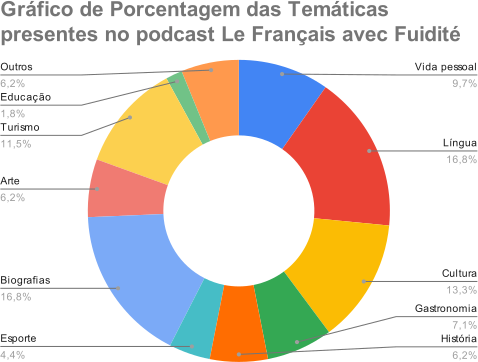
\includegraphics[width=\linewidth]{Fig1.png}
    \caption{Porcentagem das temáticas presentes no \textit{podcast Le Français avec Fluidité}.}
    \label{fig1}
    \source{Elaborado pelas autoras.}
    \end{minipage}
\end{figure}

Destacamos, nessa representação, a temática \textit{Língua}, que reúne episódios relacionados a estratégias para aprender francês (16,8\%). Na mesma proporção, encontra-se \textit{Biografias}, que se dedica à vida de celebridades da França, bem como a fatos e acontecimentos gerais de países nos quais está presente a língua francesa. Ambas as temáticas são seguidas por \textit{Cultura} (13,3\%) e \textit{Turismo} (11,5\%), sendo que os demais temas aparecem de forma menos frequente no conjunto dos dados analisados.

A partir dessa categorização, partimos para a análise do terceiro passo dos cinco C’s de Curadoria Digital, a crítica, em que o foco está na avaliação criteriosa dos materiais e a partir da qual será possível encontrar justificativas para a inclusão ou para a exclusão dos itens previamente selecionados \cite{deschaine_five_2015}. 

Interessou-nos inicialmente a categorização temática \textit{Língua}, sobretudo na série de episódios \textit{Comment parler français couramment ?}\footnote{Tradução nossa: Como falar francês fluentemente?}, por meio dos quais constatamos a valorização da variedade de prestígio do francês, a da chamada França metropolitana. A prevalência dessa posição se contrapõe aos pressupostos da educação linguística concebida nesta pesquisa, a qual “[…] deve ser pautada pela reflexão sobre o que é língua, para além de sua dimensão como sistema, e sobre o que é educação, para além da mera aquisição de um bem” \cite{grilli_por_2021}.

A partir da construção da etapa crítica, passamos para o quarto passo do processo de curadoria digital, a conceituação, ou a reorganização dos dados criticados \cite[p. 22]{deschaine_five_2015}. Nesse momento, utilizamos como ponto de partida a \Cref{fig2}, para demonstrarmos que a maioria dos vídeos (95,6\%) trata da França metropolitana, enquanto apenas 4,4\% mencionam outros países francófonos:

\begin{figure}
    \centering
    \begin{minipage}{.75\textwidth}
    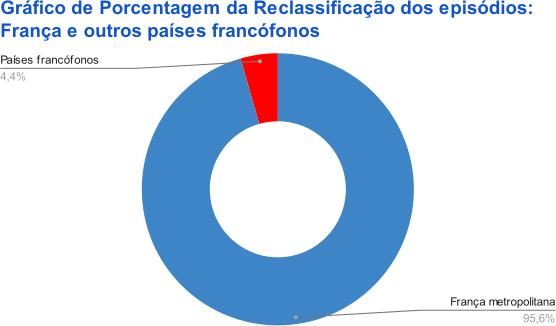
\includegraphics[width=\linewidth]{Fig2.png}
    \caption{Reclassificação dos episódios: França e outros países francófonos.}
    \label{fig2}
    \source{Elaborado pelas autoras.}
    \end{minipage}
\end{figure}

A necessidade de reclassificar os episódios em duas categorias distintas surgiu para que pudéssemos analisar de forma mais aprofundada como o apresentador aborda também a temática \textit{Cultura}, a segunda numericamente representativa após \textit{Língua} e \textit{Biografias}. Observamos, nesse caso, proporção maior de episódios referentes à França metropolitana, e é justamente a existência de outras regiões para além da linha traçada pelo apresentador que nos motivou a destacar, a seguir, a análise do episódio \textit{La France d’outre mer}.

\subsection{Crítica e conceituação: o episódio \textit{La France d’outre mer} e os atravessamentos da colonialidade da linguagem}\label{sec-fmt-manuscrito}
Destacamos os elementos do \textit{design} de \textcite{kalantzis_letramentos_2020} em nossas pesquisas entre as etapas de crítica e conceituação da curadoria digital de materiais. Reconhecemos, com essa escolha, a importância de um quadro teórico-analítico para a discussão sobre textos multimodais, em que a interação com o recurso materializado (\textit{the design} - substantivo) e o movimento de criação e agência (\textit{to design} - verbo) podem mobilizar a construção de significados na educação linguística, em nosso caso, em língua francesa.

Sob os parâmetros do quadro do design sonoro traçados por aqueles autores, analisamos o episódio \textit{La France d’outre mer}, do \textit{podcast Le Français avec Fluidité} (ver \Cref{tab01}).

\begin{table}[h!]
\centering
\begin{threeparttable}
\caption{Design sonoro ou uma gramática de significados sonoros.}
\label{tab01}
\begin{tabular}{p{2cm} p{9cm}}
\toprule
Referência & A que os significados dos sons se referem? \\
Diálogo & Como os significados dos sons conectam as pessoas que estão interagindo? \\
Estrutura & Como os significados dos sons se mantêm coesos? \\
Situação & Como os significados dos sons são moldados pelo contexto? \\
Intenção & A que interesses os significados dos sons servem? \\
\bottomrule
\end{tabular}
\source{Adaptado pelas autoras de \textcite[p. 293]{kalantzis_letramentos_2020}.}
\end{threeparttable}
\end{table}

Partindo do critério \emph{Referência}, o episódio 19, intitulado \textit{La France d’outre mer}, pode ser descrito como uma produção sonora de Fabien Sausset, com oito minutos e dez segundos de duração, disponibilizada em seu site pessoal e na plataforma Spotify.

O \textit{podcast} estabelece uma conexão entre o apresentador e o ouvinte, por meio da delimitação de quais territórios representam a França ultramarina: Guadalupe, Martinica, Saint Martin, Saint Barthélemy, Guiana Francesa, Reunião e Mayotte, Nova Caledónia, Wallis e Futuna, bem como a Polinésia Francesa. Em seguida, realiza uma breve apresentação sobre cada um deles, por meio de abordagem que recai quase exclusivamente em questões turísticas e em personalidades destacadas.

A ausência de contextualização sócio-histórica dessas regiões traz à tona a naturalização da colonização francesa sobre elas, “[...] um processo de produção e construção de um entendimento intersubjetivo da experiência da colonialidade” \cite[p. 85]{veronelli_sobre_2021} que perdura.

Além disso, poderíamos apontar que, por ser o \textit{podcast} um gênero discursivo curto e pré-gravado, a escolha de fragmentos sobre uma narrativa complexa, com o apagamento das culturas originárias daqueles territórios, não poderia  ser associada à declaração final do episódio “Agora você sabe tudo sobre a França ultramarina” (minuto 7:20)\footnote{Tradução nossa. Texto original em francês: “\textit{C’est important de le savoir parce que quand vous voyez une personne avec la peau noire en métropole, elle est : - soit d’outre mer donc française ; - soit elle vient d’anciennes colonies et elle a eu la nationalité française}”.}.

O próximo eixo do quadro de \textcite{kalantzis_letramentos_2020} – o \emph{Diálogo} – permitiu-nos reiterar a percepção de que há controle sobre as informações por meio das quais o apresentador pretende se conectar com seus ouvintes. Nessa relação de poder, ele adota abordagem seletiva ao sintetizar em um episódio dados sobre regiões ultramarinas, tratando os processos de colonização e de descolonização de maneira superficial. Isso influencia o ouvinte a adotar uma visão simplificada desses eventos históricos, promovendo “[...] o silenciamento dos sujeitos interditados comunicativamente, aludindo à racialização das populações colonizadas como agentes comunicativos, articulando, para tal colonialismo, raça, etnicidade e linguagem [...], ignorando as nuances e desafios complexos” \cite[p. 33-58]{veronelli_sobre_2021}.

A falta de implicação com essas regiões, limitadas no discurso de Fabien a curiosidades sobre turismo e celebridades, é denotada também em seu tom de fala que não se apresenta de forma expressiva, como nos episódios \textit{Apprendre sans grammaire} e \textit{La grève française}, dedicados à língua ou a aspectos da vida cotidiana francesa. No episódio em análise, a sua performance apresenta-se como monótona, sugerindo um certo desinteresse pelo conteúdo. Assim, observa-se que é dada importância apenas àquilo que o apresentador julga como crucial a ser abordado, direcionando a atenção do ouvinte para esses detalhes.

A \emph{Estrutura} do episódio é constituída por recursos sonoros, podendo ser acompanhados pela transcrição do episódio, disponível no \textit{site} do apresentador. O modo escrito é utilizado como recurso adicional e auxilia na compreensão e na acessibilidade do conteúdo para diferentes públicos, sendo veiculados inclusive em língua inglesa para quem não compreende o francês.

No que tange às características sonoras observadas ao longo do episódio, percebe-se que o ritmo adotado varia de baixo a moderado e adota uma abordagem mais pausada. Essas pausas contínuas afetam a percepção do ouvinte sobre o andamento da discussão em desenvolvimento.

Com relação à \emph{Situação} apresentada, é possível notar como a fala é enquadrada no contexto. Observa-se que significados vão sendo construídos durante a exposição do episódio. Nesse caso, destacamos a afirmação realizada pelo apresentador, diretamente de seus entendimentos eurocentrados sobre língua/cultura no contexto da discussão sobre a França ultramarina: “É importante saber disso porque, quando você vê uma pessoa com a pele negra na França metropolitana, essa pessoa é: ou da França ultramarina, portanto, francesa; ou ela vem de antigas colônias e tem a nacionalidade francesa” (6:41 min)\footnote{Tradução nossa. Texto original em francês: “\textit{C’est important de le savoir parce que quand vous voyez une personne avec la peau noire en métropole, elle est : - soit d’outre mer donc française ; - soit elle vient d’anciennes colonies et elle a eu la nationalité française}”.}. Trata-se de discurso evidentemente racista, em que a colonialidade da linguagem do apresentador reduz pessoas com suas histórias, estereotipando-as e “[...] colocando-as em situações e relações que as despojam da sua humanidade” \cite[p. 86]{veronelli_sobre_2021}.

Nesse aspecto, o episódio revisita uma problemática subjacente à forma como o conteúdo está sendo abordado na situação, de modo a influenciar as significações das falas e como elas podem afetar o público-alvo, principalmente estudantes de francês. O contexto geral do \textit{podcast}, o tópico abordado e o propósito do episódio moldam as interações e o significado das falas, uma vez que “a colonialidade condiciona o que se considera como língua humana na sua acepção plena, como as classificações da população em raças superiores e inferiores” \cite[p. 89]{veronelli_sobre_2021}. Isso ressalta a responsabilidade que deveria ser observada pelo apresentador em oferecer informações precisas e representativas, uma vez que sua influência na formação do discurso, na seleção de dados e na interpretação do conteúdo pelo público-alvo são aspectos de extrema importância ao avaliar a qualidade do diálogo apresentado.

No que se refere à \emph{Intenção}, ou às intenções, Fabien explora a temática da França ultramarina de forma reduzida, destacando apenas as questões voltadas para o turismo e personalidades conhecidas, negligenciando as questões voltadas ao contexto de colonização e descolonização dessas regiões. Sendo um falante nativo do francês, sua posição carrega consigo uma autoridade que se baseia principalmente em sua origem europeia. Assim, percebemos, como \textcite[p. 94]{veronelli_sobre_2021}, “[...] disposição da parte dos colonizadores de se comunicarem entre si enquanto reduzem possíveis interlocutores a comunicadores simples e suas linguagens a ferramentas rudimentares de expressividade”.

O apresentador desconsidera, assim, todo o contexto linguístico das regiões francesas ultramarinas e se posiciona por meio de discursos racistas e estereotipados, aceitos por sua credibilidade ser moldada pela nacionalidade francesa por meio da qual se identifica no \textit{podcast}. Essa característica tem o potencial de influenciar a percepção do ouvinte, uma vez que a autoridade do influenciador pode ser aceita sem questionamentos.

Não há dúvidas, portanto, de que a análise do episódio deflagra o quão problemática pode ser a seleção de tal conteúdo, tanto para o contexto da curadoria do/a professor/a de francês, quanto do/a estudante que utiliza tal recurso digital para o estudo dessa língua em autonomia. 

\section{Curadoria digital da plataforma \textit{Apprendre et enseigner le français avec TV5 Monde (A2)}}\label{sec-formato}
Outro trabalho sobre a curadoria digital de materiais na educação linguística que temos realizado é a investigação que se dedica à análise de vídeos da plataforma de apoio a professores/as de francês intitulada \textit{Apprendre et enseigner le français avec TV5 Monde}. 

Como se trata de um portal que disponibiliza fichas pedagógicas preparadas para a utilização por educadores/as no mundo todo, interessou-nos avaliar como são construídos os sentidos em peças fílmicas relacionadas àquelas sequências didáticas, mais especificamente em nível A2, do Quadro Comum Europeu de Referência para as Línguas.

Percorrendo também os 5 C’s de \textcite{deschaine_five_2015}, delimitamos recortes importantes sobre a veiculação do material, em especial no que tange à representação do continente africano no \textit{corpus} coletado. 

Desse modo, como na investigação anteriormente apresentada, destacaremos aqui a análise de um dos recursos digitais coletados naquela plataforma, para avaliarmos os atravessamentos que devem ser considerados quando da sua utilização em contextos de ensino-aprendizagem de francês.


\subsection{Coleção e categorização temática da plataforma \textit{Apprendre et enseigner le français avec TV5 Monde (A2)}}\label{sec-modelo}
Entre setembro e novembro de 2022, foi realizada a coleta de 381 fichas pedagógicas de nível A2, disponibilizadas no site da plataforma \textit{Apprendre et enseigner le français avec TV5 Monde} (A2). Graças a esse procedimento, foi possível identificar a prevalência do vídeo como recurso digital para o ensino-aprendizagem de francês, especialmente do videoclipe musical, conforme \Cref{fig3} 

\begin{figure}
    \centering
    \begin{minipage}{.75\textwidth}
    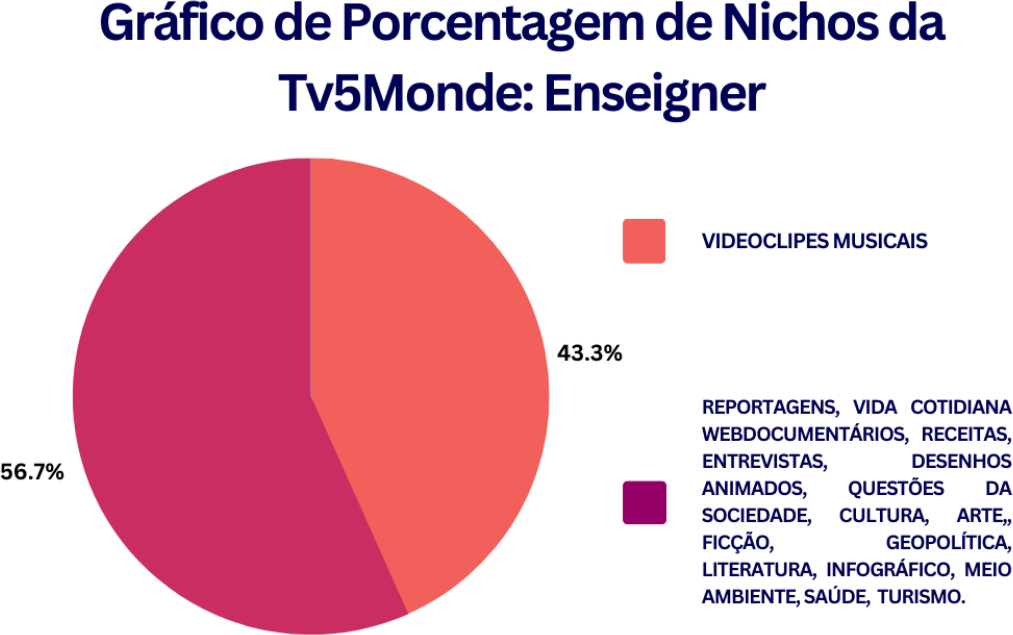
\includegraphics[width=\linewidth]{Fig3.png}
    \caption{Categorização temática dos vídeos da \textit{Apprendre et enseigner le français avec TV5 Monde} (A2).}
    \label{fig3}
    \source{Elaborado pelas autoras.}
    \end{minipage}
\end{figure}

Posteriormente, foi realizada a etapa de categorização a partir da tabulação de metadados organizados em uma planilha eletrônica, quais sejam: título da ficha, data de coleta, \textit{link} de acesso da ficha pedagógica, descrição (\textit{À propos}), data de publicação e de modificação da ficha, data limite de acesso na plataforma e possibilidade de \textit{download} do recurso digital de base (vídeo) de cada ficha. 

Desse procedimento, partiu-se para a categorização do \textit{corpus} e identificação de algumas características que atravessam a plataforma, para delimitar o recorte teórico-metodológico a ser realizado nesse universo de 381 fichas pedagógicas coletadas. A primeira delas é que apenas 109 dos vídeos vinculados a sequências didáticas de nível A2 não apresentavam restrição de data limite para \textit{download}, conforme \Cref{fig4}.

\begin{figure}
    \centering
    \begin{minipage}{.75\textwidth}
    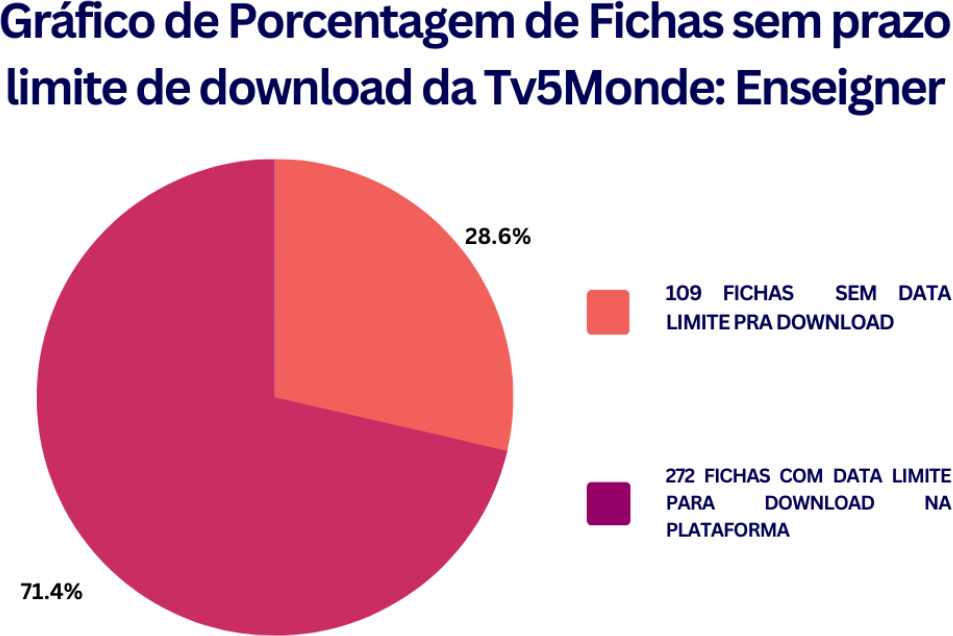
\includegraphics[width=\linewidth]{Fig4.png}
    \caption{Fichas sem prazo limite para download na plataforma \textit{Apprendre et enseigner le français avec TV5 Monde}.}
    \label{fig4}
    \source{Elaborado pelas autoras.}
    \end{minipage}
\end{figure}

Para além dessa evidente limitação do acesso livre ao conteúdo, na etapa da crítica \cite{deschaine_five_2015}, foi constatada a existência de apenas 17 fichas pedagógicas do corpus coletado, construídas em torno de webdocumentários que se referem a países africanos, como observamos no gráfico a seguir:

\begin{figure}
    \centering
    \begin{minipage}{.75\textwidth}
    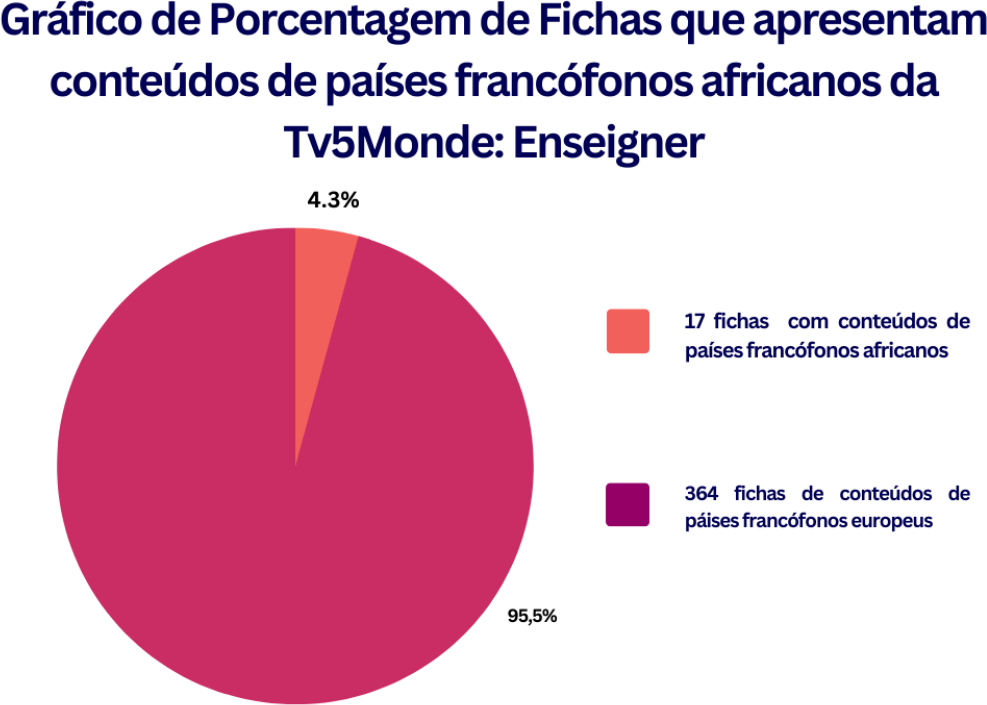
\includegraphics[width=\linewidth]{Fig5.png}
    \caption{Fichas com conteúdos de países francófonos africanos na plataforma \textit{Apprendre et enseigner le français avec TV5 Monde} (A2).}
    \label{fig5}
    \source{Elaborado pelas autoras.}
    \end{minipage}
\end{figure}

Tal constatação levou-nos a discutir a sub-representação destes territórios negros na plataforma europeia em questão, durante a etapa da conceituação a ser aprofundada na seção subsequente. Serão novamente destacados os letramentos multimodais, mais especificamente os critérios da análise do \textit{design} visual \cite{kalantzis_letramentos_2020}, mobilizados para a construção de significados de um vídeo dentre os 17 sobre África por nós identificados no \textit{corpus}. 

\subsection{Crítica e conceituação: o webdocumentário \textit{Au fast food} (Togo)}\label{sec-organizacao}
A análise dos elementos do \textit{design} de \textcite{kalantzis_letramentos_2020} também será mobilizada para a discussão do recorte aqui delimitado, mais especificamente com relação ao modo visual, por se tratar de vídeos. Sendo assim, os eixos \emph{Referência}, \emph{Diálogo}, \emph{Estrutura}, \emph{Situação} e \emph{Intenção} do quadro analítico já apresentado na seção \ref{sec-conduta} também serão aqui mencionados para destacar, na construção das fichas pedagógicas, como os elementos visuais e sonoros dos webdocumentários sobre África são articulados para influenciar a perspectiva do público da \textit{TV5Monde: Enseigner le Français}. 

Para tanto, foi selecionado o vídeo relacionado a uma ficha pedagógica intitulada \textit{Au fast food} (Togo). Trata-se de produção audiovisual do canal de serviço público franco-alemão denominado  ARTE (\textit{Association Relative à la Télévision Européenne}),  que foi fundado em 1991 e tem sede em Estrasburgo, França. 

O primeiro critério do quadro analítico diz respeito ao elemento \emph{Referência}, no qual os autores resumem a questão “O que os significados descrevem?” \cite[p. 293]{kalantzis_letramentos_2020}. Nesse caso, apontamos que o webdocumentário foi produzido por Sylvania Iorio e Anne Seymour, dirigido por Michael Unger, com os direitos reservados ao canal de origem \textit{ARTE}, com duração de 2 minutos e 32 segundos e disponível para exibição na plataforma \textit{Apprendre et enseigner le français avec TV5 Monde}.

Em sua introdução, o primeiro contato da gravação é com o movimento da rua, onde se destacam inúmeras barracas de comida de fácil acesso que formam o polo gastronômico popular de Lomé (Togo). No segundo 0:07, o narrador espera um sinal para iniciar a fala da gravação e, no segundo 0:08, começa o vídeo apresentando o \textit{fast-food} da cidade para os espectadores. Após este momento, o narrador inicia sua fala de forma irônica, afirmando, no frame 0:12, que aquelas opções de alimentação não se assemelhariam a “\textit{repas fran... européens}”. Na \Cref{fig6}, nota-se tal hesitação do narrador entre refeições francesas e europeias, até a delimitação que ocorre ao direcionar seu olhar para o cinegrafista.

\begin{figure}
    \centering
    \begin{minipage}{.75\textwidth}
    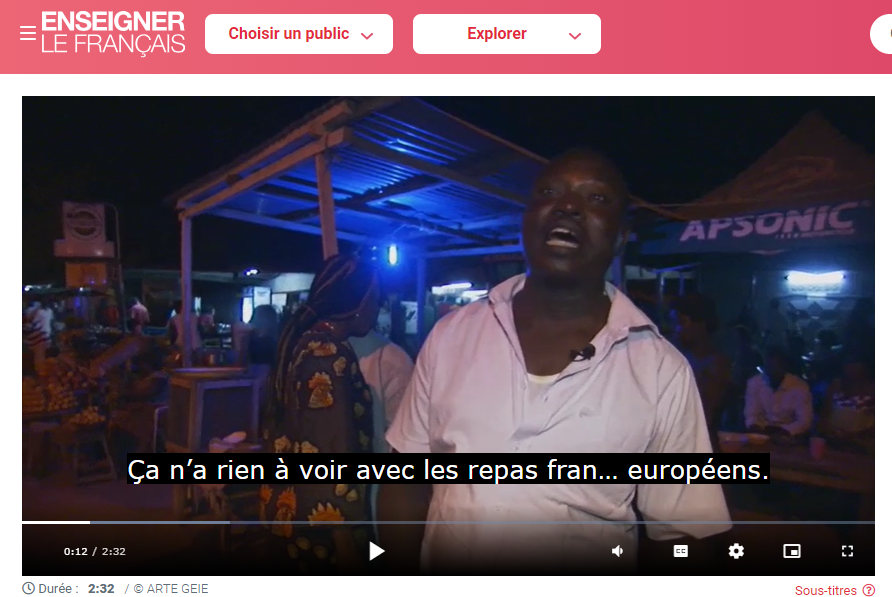
\includegraphics[width=\linewidth]{Fig6.png}
    \caption{Captura de tela sobre comparação entre refeições em Lomé (Togo).}
    \label{fig6}
    \source{Plataforma \textit{Apprendre et enseigner le français avec TV5 Monde}.}
    \end{minipage}
\end{figure}

Essa hesitação seguida de correção é importante para discutirmos o eixo \emph{Diálogo} do quadro teórico-analítico aqui adotado, por meio do qual se busca responder à questão “Como os significados conectam as pessoas que estão interagindo?” \cite[p. 293]{kalantzis_letramentos_2020}. No vídeo, a conexão entre o webdocumentário e os interlocutores é produzida com a exibição da riqueza cultural presente em Lomé, mas do ponto de vista francês e europeu, como vimos no controle da fala do apresentador pelo cinegrafista. Ao longo de sua exibição, outro morador da cidade apresenta todos os processos da confecção dos “espetos da capital” como parte da cultura local.

Além disso, o foco da câmera é de cima para baixo (\textit{plongée}) para exibição de detalhes das cenas: os nomes das barracas, o modo de produção dos espetinhos, as mulheres no processo de produção do alimento, com suas \textit{capulanas}, tecidos coloridos utilizado para vários fins, como turbante, roupas e carregadores de bebês, como no caso da mulher na cena, trabalhando acompanhada de sua criança colada ao corpo (\Cref{fig7}).

\begin{figure}
    \centering
    \begin{minipage}{.75\textwidth}
    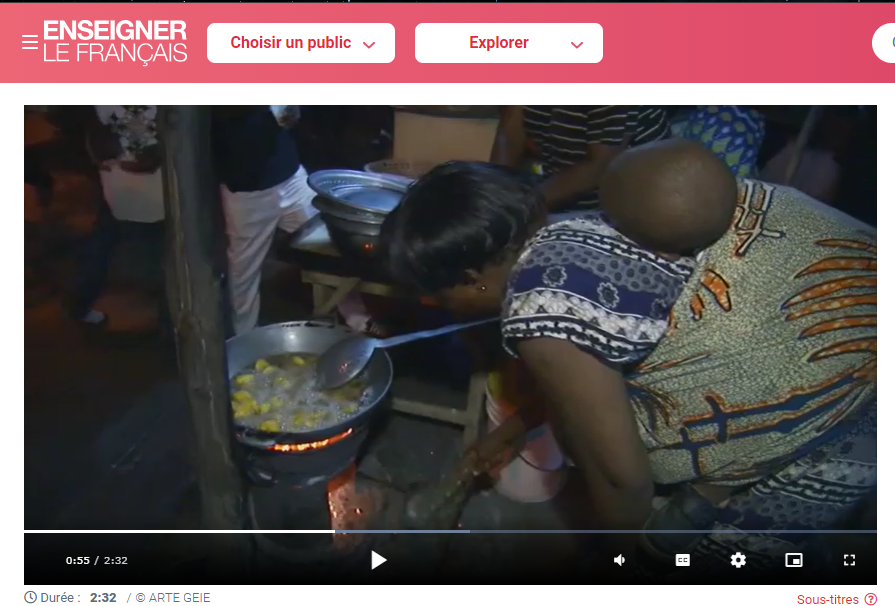
\includegraphics[width=\linewidth]{Fig7.png}
    \caption{Mulher com sua criança em barraca de comida (Lomé, Togo).}
    \label{fig7}
    \source{Plataforma \textit{Apprendre et enseigner le français avec TV5 Monde}.}
    \end{minipage}
\end{figure}

De igual modo, no decorrer da filmagem, é possível perceber um número expressivo de motocicletas passando por trás da câmera, além de muitas buzinas. As barracas de espeto filmadas durante todo o vídeo também exibem \textit{takes} do alimento na grelha. O cinegrafista prioriza a correria do trabalho realizado em um ambiente quase impossível de haver comunicação e, nesses instantes, é possível notar o foco no comércio local de Togo como curioso, como se a equipe europeia fosse a desbravadora de uma realidade exótica. Ademais, o webdocumentário é acompanhado por uma música africana sobre a qual não se tem acesso nos créditos ao nome, compositor e cantor.

A \emph{Estrutura}, elemento que se refere à questão “Como os significados em geral se mantêm juntos?” \cite[p. 293]{kalantzis_letramentos_2020}, na análise do webdocumentário reproduzido, possui tanto elementos constituintes em formato de imagem, quanto sons, sendo também acompanhados de legendas ativadas ou não, o que eventualmente ajuda o público a compreender o conjunto dos recursos do vídeo. Na finalização e edição, foram mantidos diálogos entre apresentadores (narradores locais) e o cinegrafista que conduz o trajeto e o foco da câmera no polo gastronômico de  Lomé. 

Quando se fala em Situação, deseja-se saber “como os significados são moldados pelo seu contexto” \cite[p. 293]{kalantzis_letramentos_2020}. Como um critério analítico, os protagonistas da cena mostram-se à vontade ao serem filmados, mesmo exercendo um trabalho exaustivo de 24 horas, como demonstramos na \Cref{fig8}:

\begin{figure}
    \centering
    \begin{minipage}{.75\textwidth}
    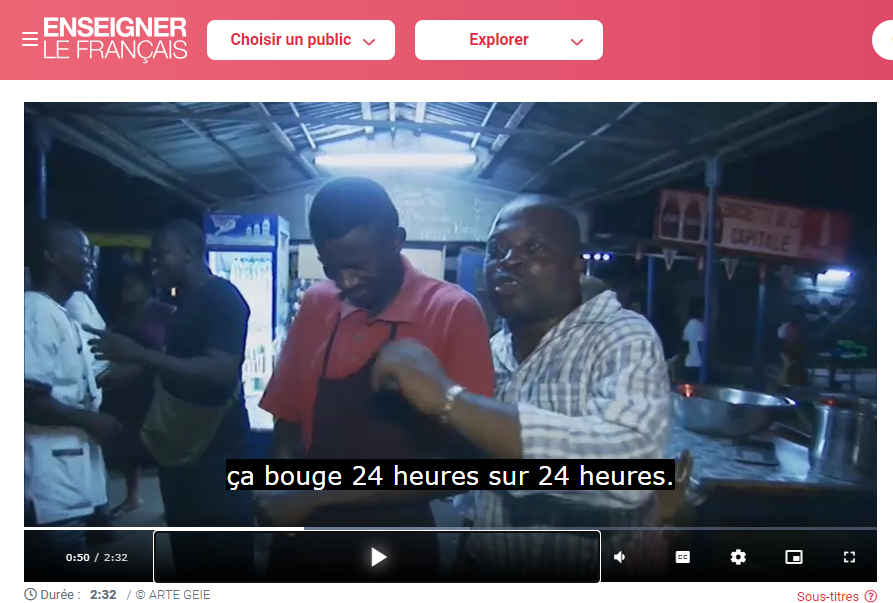
\includegraphics[width=\linewidth]{Fig8.png}
    \caption{Captura de tela com comentário sobre o trabalho ininterrupto no polo gastronômico de Lomé, Togo.}
    \label{fig8}
    \source{Plataforma \textit{Apprendre et enseigner le français avec TV5 Monde}.}
    \end{minipage}
\end{figure}

O sentimento de orgulho parece presente, mas quando sua cultura gastronômica é apresentada à câmera, fala prioritariamente para telespectadores europeus, aos quais o trabalho nos trópicos ressurge como a naturalização da exploração colonial dos corpos pretos, memória que ressurge na legenda “\textit{24 heures sur 24 heures}”. 

No que se refere à \emph{Intenção} do material, ou “A que propósitos e interesses esses significados são destinados a servir?” \cite[p. 293]{kalantzis_letramentos_2020}, o webdocumentário serve ao interesse do público europeu do canal, que busca transmitir o comércio gastronômico popular de Lomé por guias locais, contratados pela \textit{ARTE}. O foco não está em considerar uma culinária representativa da cidade de Lomé, apresentando para espectadores de fora da realidade de Togo uma conexão com as raízes ancestrais, em que a construção de identidade e fortalecimento transporta o reconhecimento do continente africano como uma extensão territorial rica e diversa. Ao contrário, quando produzem e exibem produções no viés aqui apontado, a plataforma reafirma a narrativa discursiva monolítica associada à África, conduzindo uma visão e relação de poder ligadas ao imaginário colonizador/colonizado.

Mesmo sendo uma jornada exaustiva, durante a qual o trabalho massante ocorre pela sobrevivência, este mesmo trabalho de “\textit{24 heures sur 24 heures}” é exibido para os espectadores como divertido e exótico. Nesse enfoque, o uso do quadro de análise dos elementos do design de \textcite{kalantzis_letramentos_2020} se faz essencial, desvelando o olhar eurocentrado para culturas de territórios africanos, por meio de produção de conteúdo e roteiro controlados.

Dessa forma, quando se trata de intenção, é necessário reiterar a presença do cinegrafista, notando sua orientação em todos os instantes do webdocumentário para dirigir a forma como os guias apresentam e falam diante da câmera. Nesse sentido, a repetição de vários \textit{takes}, percebidos pela frequência de cortes, endossam a existência de um roteiro programado, mesmo que os momentos iniciais do vídeo simulem uma construção espontânea e natural. Isso poderia gerar uma produção de material midiático supostamente ingênua, o que se demonstrou em frames nos quais as expressões faciais dos apresentadores se direcionam com hesitação ao expressarem algumas falas, muitas vezes interrompidas no corte de cena.

Constatamos, especialmente nos últimos segundos de vídeo, que o guia/apresentador do início do webdocumentário retorna à cena, sendo instruído pelo cinegrafista a ingerir álcool nas gravações. É, então, interrompido na sua finalização de fala, que é refeita diversas vezes, conforme \Cref{fig9}.

\begin{figure}
    \centering
    \begin{minipage}{.75\textwidth}
    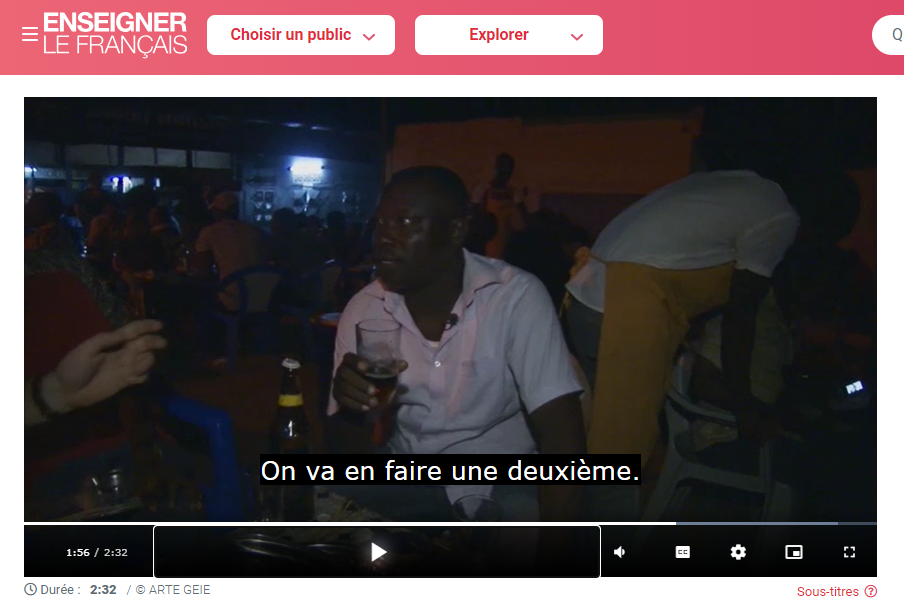
\includegraphics[width=\linewidth]{Fig9.png}
    \caption{Captura de tela com interferência de cinegrafista em cena na qual um apresentador local de Tomé ingere bebida alcoólica.}
    \label{fig9}
    \source{Plataforma \textit{Apprendre et enseigner le français avec TV5 Monde}.}
    \end{minipage}
\end{figure}

Em outra cena, o mesmo apresentador é ainda orientado pelo cinegrafista a tomar um gole maior da bebida (\textit{bonne gorgée}) (Ver \Cref{fig10}).

\begin{figure}
    \centering
    \begin{minipage}{.75\textwidth}
    
\includegraphics[width=\linewidth]{Fig10.png}
    \caption{Cena na qual um apresentador local de Tomé é orientado a tomar um gole maior de bebida (\textit{bonne gorgée}).}
    \label{fig10}
    \source{Plataforma \textit{Apprendre et enseigner le français avec TV5 Monde}.}
    \end{minipage}
\end{figure}

O modo particularmente significativo pelo qual a entoação do cinegrafista se manifesta na descrição da legenda como voz \textit{off} revela que a intenção de exibir os guias em um estado de embriaguez foi cuidadosamente projetada e executada pelo canal ARTE e pela equipe de produção do vídeo. Essa abordagem ressurge, mais uma vez, para conceder ao homem europeu uma posição de deleite diante de cenas em que corpos negros são alvo de zombaria, reforçando a associação entre a sua identidade étnico-racial e o alcoolismo.

Essa associação, especialmente no contexto de trabalho, acaba perpetuando a ideia de ociosidade ligada aos corpos negros, além de forçar uma percepção de felicidade que não acontece genuinamente durante as filmagens. O trabalho exaustivo dos vendedores de “espetinhos da capital” é exibido de forma prazerosa, vindo a camuflar o cansaço físico e mental de uma atividade exercida sem descanso para a manutenção da sobrevivência. 

Desse modo, a curadoria desse conteúdo para uso em situações de ensino-aprendizagem de francês também precisa ser discutida sob lentes decoloniais que ampliem os atravessamentos já discutidos por nós quando sobre a permanência da colonialidade da linguagem \cite{veronelli_sobre_2021}. No caso aqui em destaque, é preciso nomear também como racista o recorte ostensivo realizado sobre as vivências do povo de Lomé, lidas pelo público-alvo branco e europeu do canal \textit{ARTE} e da plataforma \textit{Apprendre et enseigner le français avec TV5 Monde}.


\section{Conclusão}\label{sec-organizacao-latex}
Em ambas as pesquisas situadas no contexto em que investigamos o processo de curadoria digital de materiais entre futuros professores/as de francês na Universidade Federal do Piauí, buscou-se analisar limites e possibilidades do \textit{podcast Le Français avec Fluidité} e da plataforma \textit{Apprendre et enseigner le français avec TV5 Monde} para a promoção de desenhos didáticos éticos e estéticos \cite{rocha_moocs_2019}. 

Os atravessamentos da colonialidade da linguagem se destacaram nos recortes analíticos aqui expostos, que se realizaram à luz de quadro representativo do \textit{design} sonoro, para a discussão sobre um episódio daquele \textit{podcast}, e visual, para o webdocumentário.  

A pesquisa deve ser ainda ampliada, porém o movimento aqui realizado já sinaliza o primeiro passo rumo à etapa da circulação (crítica) dos materiais que analisamos. A divulgação deste trabalho fomentará, certamente, a necessidade de traçarmos referenciais para a curadoria digital que sejam decoloniais e antirracistas, visando à formação do/a professor/a de línguas em seu processo como curador/a-criador/a de materiais didáticos na educação linguística.

\printbibliography\label{sec-bib}
% if the text is not in Portuguese, it might be necessary to use the code below instead to print the correct ABNT abbreviations [s.n.], [s.l.]
%\begin{portuguese}
%\printbibliography[title={Bibliography}]
%\end{portuguese}


%full list: conceptualization,datacuration,formalanalysis,funding,investigation,methodology,projadm,resources,software,supervision,validation,visualization,writing,review
\begin{contributors}[sec-contributors]
	\authorcontribution{Marcella dos Santos Abreu}[conceptualization,methodology,validation,projadm,supervision,visualization,writing,review]
	\authorcontribution{Lorrana Crystina da Costa Dias}[conceptualization,datacuration,investigation]
	\authorcontribution{Maria Eduarda de Sousa Oliveira}[conceptualization,datacuration,investigation]
\end{contributors}


\end{document}

